\documentclass[11pt,a4paper]{article}

\usepackage[utf8]{inputenc}
\usepackage[T1]{fontenc}
\usepackage{lmodern}
\usepackage[margin=2.5cm]{geometry}
\usepackage{graphicx}
\usepackage{booktabs}
\usepackage{tabularx}
\usepackage{longtable}
\usepackage{enumitem}
\usepackage{hyperref}
\usepackage{xcolor}
\usepackage{titlesec}
\usepackage{fancyhdr}
\usepackage{parskip}
\usepackage{tikz}

% Colors matching Spotree brand
\definecolor{spotgreen}{HTML}{2d6a4f}
\definecolor{spotlight}{HTML}{52b788}
\definecolor{spotbg}{HTML}{f0fdf4}
\definecolor{spotdark}{HTML}{1b4332}
\definecolor{spotgray}{HTML}{666666}

% Hyperlink styling
\hypersetup{
  colorlinks=true,
  linkcolor=spotgreen,
  urlcolor=spotgreen,
  citecolor=spotgreen,
  pdftitle={Spotree -- Proposal for TreeQuest Challenge},
  pdfauthor={Spotree Team}
}

% Section styling
\titleformat{\section}{\Large\bfseries\color{spotdark}}{}{0em}{}[\vspace{-0.5em}\textcolor{spotlight}{\rule{\textwidth}{1.5pt}}]
\titleformat{\subsection}{\large\bfseries\color{spotgreen}}{}{0em}{}
\titleformat{\subsubsection}{\normalsize\bfseries\color{spotdark}}{}{0em}{}

% Header/footer
\pagestyle{fancy}
\fancyhf{}
\fancyhead[L]{\small\color{spotgray}Spotree -- TreeQuest Challenge Proposal}
\fancyhead[R]{\small\color{spotgray}\thepage}
\fancyfoot[C]{\small\color{spotgray}Munich Innovation Challenge 2025}
\renewcommand{\headrulewidth}{0.4pt}
\renewcommand{\footrulewidth}{0.4pt}

\begin{document}

% ── Title Page ──
\begin{titlepage}
\centering
\vspace*{3cm}

{\Huge\bfseries\color{spotdark} Spotree\par}
\vspace{0.5cm}
{\Large\color{spotlight} Spotify + Tree Mapping\par}
\vspace{1.5cm}
{\large\bfseries Proposal for the TreeQuest Challenge\par}
\vspace{0.5cm}
{\large Munich Innovation Challenge\par}
{\large\color{spotgray} Students on an Urban Data Mission\par}

\vspace{2cm}


\begin{tikzpicture}
\draw[spotgreen, line width=2pt] (0,0) -- (12,0);
\end{tikzpicture}

\vspace{2cm}

{\large\color{spotgray} Submitted by the Spotree Team\par}
\vspace{0.5cm}
{\color{spotgray} May 2025\par}

\vfill
\end{titlepage}

% ── Table of Contents ──
\tableofcontents
\newpage

% ══════════════════════════════════════════════════════════════
\section{Team}

\begin{center}
\begin{tabularx}{\textwidth}{l l X}
\toprule
\textbf{Name} & \textbf{Role} & \textbf{Background} \\
\midrule
 &  &  \\
 &  &  \\
\bottomrule
\end{tabularx}
\end{center}

\textit{[To be filled by team members]}

% ══════════════════════════════════════════════════════════════
\section{Executive Summary}

\textbf{Spotree} (Spotify + Tree) is a mobile application that transforms urban tree mapping into an engaging, social experience for Munich's students. Instead of treating data collection as a chore, Spotree lets students ``spot'' trees, capture rich geospatial data, and \textbf{drop their favorite Spotify song at each tree location} --- creating a musical map of Munich's urban forest.

The name says it all: \textbf{Spo}(tify) + \textbf{tree}. Every tree becomes a point on the map with a soundtrack. When students explore trees mapped by their peers, they can tap to play the linked song. This social, music-driven mechanic gives students a personal reason to keep mapping --- they want to see their song on the map, share it with friends, and discover what others have linked. It turns a civic data project into something students genuinely want to participate in.

Behind the fun interface, Spotree builds a \textbf{production-grade geospatial database} using PostGIS with OGC-compliant spatial data types, ready for direct integration into Munich's existing geodata infrastructure.

% ══════════════════════════════════════════════════════════════
\section{Challenge Response}

The challenge asks: \textit{How can we involve students in Munich in the creation and updating of the city's geospatial data in an active and educational way, while strengthening their connection to their neighbourhood?}

Spotree addresses every dimension of this question:

\begin{center}
\small
\begin{tabularx}{\textwidth}{>{\bfseries}l X}
\toprule
\textbf{Challenge Requirement} & \textbf{Spotree Solution} \\
\midrule
Crowdsourced data collection & Students capture tree photos, GPS-tagged locations, species identification, health assessment, height estimation, and trunk diameter --- all through a guided mobile form \\
\addlinespace
Educational value & The Spotree Guide teaches 58 native Munich tree species with photos, growth characteristics, habitat info, and links to botanical references (Easyscape). Students learn to identify species before they map \\
\addlinespace
Active participation & The Spotify integration creates intrinsic motivation. Students map trees to drop songs. School-level analytics enable teachers to integrate mapping into lessons \\
\addlinespace
AI integration & Current prototype uses AI (LLaVA vision model) to validate uploaded photos contain trees. Co-creation phase adds AI-powered species classification \\
\addlinespace
Neighbourhood connection & Students explore trees in their area, discover songs left by peers, and build a personal profile. The map becomes a living, musical portrait of their neighbourhood \\
\addlinespace
Rewarding / ranking & Profile tracks trees spotted, species found, and songs shared. Co-creation phase adds leaderboards and area ownership mechanics \\
\addlinespace
OGC-compliant data & All spatial data stored as PostGIS \texttt{geography(Point, 4326)} --- standard WGS84. Export to GeoJSON, Shapefile, GeoParquet supported natively \\
\addlinespace
Verification \& updates & AI rejects non-tree photos. Confidence sliders on every field signal data quality. Multiple students can map the same tree, enabling cross-verification \\
\bottomrule
\end{tabularx}
\end{center}

% ══════════════════════════════════════════════════════════════
\section{App Description}

Spotree is built as a native iOS app (React Native + Expo) with 5 main tabs:

\subsection{Map}
The central view showing all spotted trees across Munich on an interactive map. Each tree marker indicates its location; markers with a music badge have a linked Spotify song. Tapping a marker opens a detail card showing species, health, height, who mapped it, and a play button for the linked song.

\subsection{Capture (Spot a Tree)}
The guided data collection form. Students can:
\begin{itemize}[nosep]
  \item \textbf{Take a photo} (camera) or \textbf{pick from gallery} (with EXIF GPS extraction)
  \item AI validates the photo contains a tree before proceeding
  \item Select \textbf{tree species} from 58 Munich natives (or ``Not Sure'' if uncertain)
  \item Rate \textbf{health status} (Healthy / Fair / Poor / Dead)
  \item Estimate \textbf{tree height} and \textbf{trunk diameter}
  \item Set \textbf{confidence levels} (0--100\%) for each observation via sliders
  \item Add \textbf{free-text notes} about the tree or its surroundings
  \item \textbf{Link a Spotify song} --- paste a URL and name the track
\end{itemize}

After submission, the tree appears on the map for all users.

\subsection{Explore}
A social feed of recently spotted trees, sorted by time. Each card shows the tree photo, species, health, height, confidence bar, mapper's name, and linked song with a play button. A \textbf{``View on Map''} button zooms directly to any tree's location on the map.

\subsection{Spotree Guide}
An educational reference for Munich's native tree species:
\begin{itemize}[nosep]
  \item \textbf{58 species} with common and scientific names
  \item \textbf{Swipeable image galleries} with multiple photos per species
  \item \textbf{Fullscreen image viewer} for detailed examination
  \item Plant description chips: height, width, growth rate, flower color, blooming season, leaf retention
  \item Growth requirements: sun exposure, drainage needs
  \item Natural habitat description and common uses
  \item \textbf{External link to Easyscape} for deeper botanical learning
\end{itemize}

Data sourced from Easyscape, a botanical reference platform with verified species information.

\subsection{Profile}
Personal dashboard showing:
\begin{itemize}[nosep]
  \item \textbf{Trees Spotted} --- total count
  \item \textbf{Songs Shared} --- trees with linked songs
  \item \textbf{Species Found} --- unique species identified
  \item List of all personally mapped trees with dates and health status
  \item School affiliation (set once during registration)
\end{itemize}

% ══════════════════════════════════════════════════════════════
\section{Data Collection \& Value for GeodataService Munich}

Every tree entry in Spotree captures a comprehensive dataset designed to be directly useful for Munich's GeodataService:

\begin{center}
\small
\begin{tabularx}{\textwidth}{l l X}
\toprule
\textbf{Field} & \textbf{Type} & \textbf{Purpose} \\
\midrule
GPS Location & PostGIS Point (4326) & Precise tree position from camera GPS or EXIF metadata \\
Photo & Image URL & Visual verification of tree existence and condition \\
Species & Text (58 natives) & Tree species identification \\
Species Confidence & Integer (0--100\%) & Self-assessed certainty --- signals data quality \\
Health Status & Enum & Current tree condition (Healthy/Fair/Poor/Dead) \\
Health Confidence & Integer (0--100\%) & Certainty of health assessment \\
Estimated Height & Text (ranges) & Approximate tree height \\
Height Confidence & Integer (0--100\%) & Certainty of height estimate \\
Trunk Diameter & Text (ranges) & Approximate diameter at breast height \\
Diameter Confidence & Integer (0--100\%) & Certainty of diameter estimate \\
Notes & Free text & Additional observations (damage, surroundings, etc.) \\
Timestamp & ISO 8601 & When the observation was recorded \\
User \& School & Reference & Who collected the data and from which school \\
\bottomrule
\end{tabularx}
\end{center}

The \textbf{confidence sliders are a key design decision}. Rather than forcing students to guess, they can honestly mark uncertainty. This gives GeodataService a built-in quality metric: a tree with 90\% species confidence from three students is far more reliable than a single observation at 30\%. This enables quality-weighted data integration.

\textbf{School-level tracking} allows GeodataService to understand geographic coverage patterns --- which neighborhoods are well-mapped based on which schools participate. This helps identify gaps and target outreach.

% ══════════════════════════════════════════════════════════════
\section{AI Integration}

\subsection{Current Prototype: Image Validation}
The prototype implements AI-powered photo validation to ensure data quality:

\begin{enumerate}[nosep]
  \item Student takes or selects a photo
  \item Photo is resized (512px) and base64-encoded on-device
  \item Sent to a \textbf{Cloudflare Worker proxy} (server-side, no API keys exposed to client)
  \item The Worker calls \textbf{LLaVA 1.5}, a vision-language model, which generates a natural language description of the image
  \item Description is checked for tree-related keywords (tree, trunk, bark, branch, canopy, etc.)
  \item Non-tree images are rejected with a clear message
\end{enumerate}

This prevents misuse and ensures every entry in the database actually represents a tree.

\subsection{Co-Creation Phase: Species Classification}
See Section~\ref{sec:ai-species} for the planned AI species identification system with continuous learning.

% ══════════════════════════════════════════════════════════════
\section{Technical Architecture}

\begin{center}
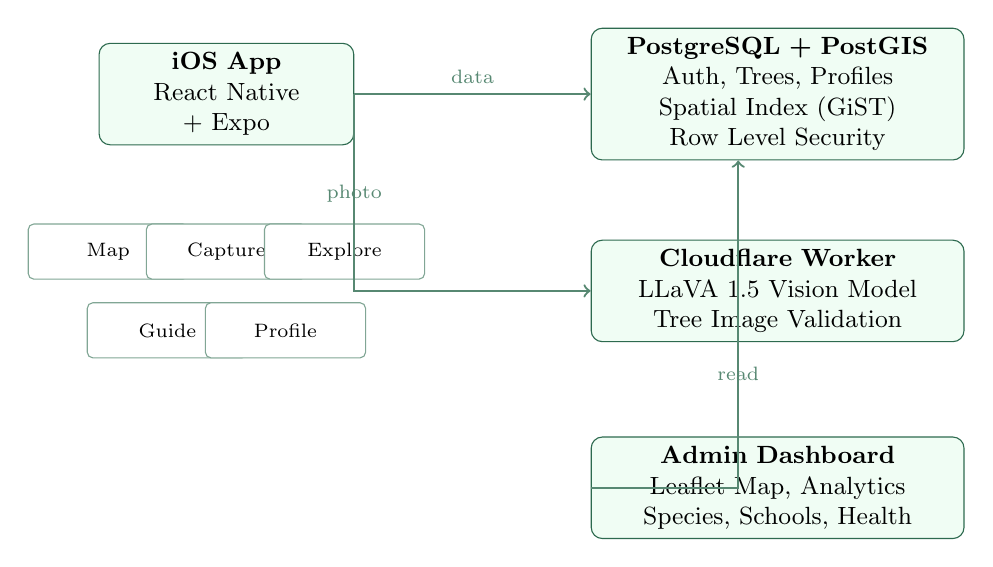
\begin{tikzpicture}[
  box/.style={draw=spotgreen, fill=spotbg, rounded corners=4pt, minimum height=1.2cm, text width=4cm, align=center, font=\small},
  smallbox/.style={draw=spotgreen!60, fill=white, rounded corners=2pt, minimum height=0.7cm, text width=2.8cm, align=center, font=\scriptsize},
  arrow/.style={->, thick, spotgreen!80},
  every node/.style={font=\small}
]

% iOS App
\node[box, text width=3cm] (app) at (0, 0) {\textbf{iOS App}\\React Native\\+ Expo};

% Screens
\node[smallbox, text width=1.8cm] (map) at (-1.5, -2) {Map};
\node[smallbox, text width=1.8cm] (cap) at (0, -2) {Capture};
\node[smallbox, text width=1.8cm] (exp) at (1.5, -2) {Explore};
\node[smallbox, text width=1.8cm] (gui) at (-0.75, -3) {Guide};
\node[smallbox, text width=1.8cm] (pro) at (0.75, -3) {Profile};

% Backend
\node[box, text width=4.5cm] (db) at (7, 0) {\textbf{PostgreSQL + PostGIS}\\Auth, Trees, Profiles\\Spatial Index (GiST)\\Row Level Security};

% AI
\node[box, text width=4.5cm] (ai) at (7, -2.5) {\textbf{Cloudflare Worker}\\LLaVA 1.5 Vision Model\\Tree Image Validation};

% Admin
\node[box, text width=4.5cm] (admin) at (7, -5) {\textbf{Admin Dashboard}\\Leaflet Map, Analytics\\Species, Schools, Health};

% Arrows
\draw[arrow] (app.east) -- node[above, font=\scriptsize] {data} (db.west);
\draw[arrow] (app.east) |- node[above, font=\scriptsize, pos=0.3] {photo} (ai.west);
\draw[arrow] (admin.west) -| node[below, font=\scriptsize, pos=0.7] {read} ([xshift=-0.5cm]db.south);

\end{tikzpicture}
\end{center}

\subsection{Tech Stack}

\begin{center}
\begin{tabularx}{\textwidth}{l X}
\toprule
\textbf{Component} & \textbf{Technology} \\
\midrule
Mobile App & React Native + Expo SDK 54, TypeScript \\
Authentication & Supabase Auth (email/password) \\
Database & PostgreSQL + PostGIS (via Supabase) \\
Spatial Data & \texttt{geography(Point, 4326)} with GiST spatial index \\
AI Validation & Cloudflare Workers AI --- LLaVA 1.5 vision-language model \\
AI Proxy & Cloudflare Worker (keeps API keys server-side) \\
Image Processing & expo-image-manipulator (resize/compress before AI) \\
Maps (App) & react-native-maps (Apple Maps / Google Maps) \\
Maps (Admin) & Leaflet.js + CARTO dark tile layer \\
Admin Dashboard & Single-file HTML/JS --- zero build step \\
\bottomrule
\end{tabularx}
\end{center}

% ══════════════════════════════════════════════════════════════
\section{Admin Analytics Dashboard}

The admin dashboard is a web application designed for teachers, city administrators, and GeodataService staff to monitor the project at a glance. It connects to the same database as the mobile app and displays live data.

\textbf{Layout:} Stats panel on the left, full interactive map on the right --- no scrolling needed. Grafana-inspired dark theme for comfortable monitoring.

\textbf{Panels:}
\begin{itemize}[nosep]
  \item \textbf{Stats Strip} --- Total trees, registered users, unique species found, songs linked (with weekly deltas)
  \item \textbf{Species Breakdown} --- Ranked list of all identified species with distribution bars
  \item \textbf{School Analytics} --- Trees per school, showing which schools are most actively participating
  \item \textbf{Health Overview} --- Distribution of tree health statuses across all observations
  \item \textbf{Activity Feed} --- Real-time stream of the latest tree submissions with timestamps, species, and linked songs
  \item \textbf{Interactive Map} --- All trees plotted on a dark-themed map with popups showing full details
\end{itemize}

\textbf{School-level analytics} are particularly valuable: they show which schools and neighborhoods are actively engaged, help identify coverage gaps, and enable targeted outreach to underrepresented areas.

% ══════════════════════════════════════════════════════════════
\section{OGC Compliance \& Data Export}

All tree data is stored in a \textbf{PostGIS} database using the standard \texttt{geography(Point, 4326)} type --- WGS84 coordinate reference system, the global standard for GPS data and OGC-compliant spatial systems.

This means the data can be exported directly in standard GIS formats:

\begin{center}
\begin{tabularx}{\textwidth}{l l X}
\toprule
\textbf{Format} & \textbf{Method} & \textbf{Use Case} \\
\midrule
GeoJSON & \texttt{ST\_AsGeoJSON()} or API & Web mapping, API integration, lightweight exchange \\
Shapefile & \texttt{pgsql2shp} or QGIS & Traditional GIS software (ArcGIS, QGIS), municipal systems \\
GeoParquet & \texttt{ogr2ogr} with Parquet driver & Modern columnar format for large-scale spatial analytics \\
WFS/WMS & GeoServer or pg\_featureserv & OGC web services for SDI infrastructure integration \\
\bottomrule
\end{tabularx}
\end{center}

The database schema uses a \textbf{spatial index} (GiST) on the tree locations for efficient spatial queries --- bounding box lookups, nearest-neighbor searches, and spatial joins with existing Munich geodata layers.

\textbf{Integration path:} Munich's GeodataService can connect directly to the PostGIS database via standard drivers, or consume exported files in their preferred format. The \texttt{trees\_with\_user} view provides a clean, denormalized dataset ready for analysis.

% ══════════════════════════════════════════════════════════════
\section{Screenshots}

\textit{[Insert screenshots of the following screens]}

\begin{enumerate}[nosep]
  \item \textbf{Login Screen} --- Spotree branding with sign-in form
  \item \textbf{Map View} --- Tree markers across Munich with music badges
  \item \textbf{Tree Detail Modal} --- Species, health, mapper info, Spotify play button
  \item \textbf{Capture Form} --- Photo section with AI validation, species picker, confidence sliders, Spotify link
  \item \textbf{Explore Feed} --- Social feed of recent trees with ``View on Map'' buttons
  \item \textbf{Spotree Guide} --- Species grid with image galleries
  \item \textbf{Species Detail Card} --- Full info card with carousel, growth data, habitat
  \item \textbf{Profile} --- Personal stats, tree list, school affiliation
  \item \textbf{Admin Dashboard} --- Full Grafana-style analytics view with map
\end{enumerate}

% ══════════════════════════════════════════════════════════════
\section{Co-Creation Phase Roadmap}

The current prototype demonstrates the core concept and technical feasibility. The co-creation phase will expand Spotree into a production-ready platform.

\subsection{Gamification \& Reward System}

\textbf{Leaderboard:} A public ranking of top contributors by trees spotted, species identified, and data quality (based on confidence scores and verification by other students). Visible in-app to drive friendly competition.

\textbf{Area Ownership:} Students can ``own'' a neighborhood zone (by postal code) by being the top contributor in that area. If another student maps more trees or provides higher-quality data in the same zone, ownership transfers. This creates ongoing engagement --- students return to defend their territory and fill in gaps. It directly addresses the challenge goal of strengthening neighbourhood connection: students develop a sense of responsibility for ``their'' zone's tree data.

\textbf{Badges \& Milestones:} Unlock achievements for first tree, first species ID, mapping in multiple neighborhoods, seasonal mapping (capturing the same tree across seasons), etc.

\subsection{AI-Powered Species Classification}
\label{sec:ai-species}

The current prototype uses AI to validate that photos contain trees. The co-creation phase will add \textbf{automatic species identification}:

\subsubsection{Approach}
\begin{enumerate}[nosep]
  \item \textbf{Ground truth collection} --- Use the prototype to collect GPS-tagged, species-labeled photos from students. Each photo has a species label and confidence score, giving us a quality-weighted training dataset.
  \item \textbf{Seasonal variation} --- Munich trees look significantly different across seasons (leaf-on vs.\ leaf-off, flowering periods, autumn colors). We will systematically collect images across all four seasons. A model trained only on summer photos would fail in winter.
  \item \textbf{Munich-specific training} --- Urban trees in Munich may look different from the same species in a forest or another climate zone. Local training data ensures the model reflects actual conditions.
  \item \textbf{Model options:}
  \begin{itemize}[nosep]
    \item Fine-tune an open-source vision model on Munich-specific data
    \item Evaluate existing providers (Pl@ntNet API, iNaturalist model) for baseline accuracy
    \item Focus custom training on species where existing models struggle
  \end{itemize}
  \item \textbf{In-app flow:} After the student takes a photo, the AI suggests a species with a confidence score. The student can accept, correct, or mark as ``Not Sure.'' Corrections feed back into the training loop.
\end{enumerate}

\subsubsection{Continuous Learning from Student Data}

Every tree submitted through Spotree becomes a potential training sample. The species label paired with the student's confidence score acts as a \textbf{soft label} --- a submission with 95\% confidence is a stronger training signal than one at 40\%. As the database grows, we can:

\begin{itemize}[nosep]
  \item Filter high-confidence submissions (e.g., $>$80\%) as reliable ground truth for model retraining
  \item Use cross-verified entries (same tree, same species from multiple students) as gold-standard labels
  \item Retrain or fine-tune the model periodically with the latest data, so it improves as more students contribute
  \item Track model accuracy over time by comparing AI predictions against student consensus
\end{itemize}

This creates a \textbf{virtuous cycle}: students collect data, data trains the model, the model helps future students identify species more accurately, and those students submit even better-labeled data. The more Spotree is used, the smarter it gets.

\subsection{Educational Earth Observation Module}

A new tab in the Spotree Guide showing \textbf{how tree species appear from different sensors and perspectives:}

\begin{itemize}[nosep]
  \item \textbf{High-resolution satellite imagery} --- What does a cluster of this species look like from orbit? (Using freely available Sentinel-2 or commercial VHR imagery)
  \item \textbf{Hyperspectral views} --- How does the spectral signature of this species differ from others? This introduces students to the concept that sensors can ``see'' beyond visible light
  \item \textbf{LiDAR point clouds} --- 3D structure of tree canopies, connecting to the height and diameter measurements students make on the ground
  \item \textbf{Seasonal comparisons} --- Same location across seasons from satellite, showing phenological changes
\end{itemize}

This bridges the gap between ground-level observation and remote sensing, introducing students to how cities actually monitor urban forests at scale. Space and satellite technology is inherently exciting for students and adds a unique educational dimension beyond traditional biology lessons.

\subsection{Platform Scalability}

The Spotree architecture is \textbf{not limited to trees}. The same capture-validate-map-explore pattern can be extended to other urban assets:

\begin{itemize}[nosep]
  \item \textbf{Public benches} --- location, condition, accessibility
  \item \textbf{Table tennis tables} --- public sports infrastructure mapping
  \item \textbf{Playgrounds} --- equipment inventory and condition
  \item \textbf{Street furniture} --- bike racks, waste bins, public art
\end{itemize}

Each asset type gets its own capture form, guide section, and map layer. The database schema, admin dashboard, and gamification system remain the same. This makes Spotree a general-purpose \textbf{crowdsourced urban data collection platform} that starts with trees and grows with the city's needs.

\subsection{Production Infrastructure}

The current prototype runs on Supabase's free tier. For production deployment:

\begin{center}
\begin{tabularx}{\textwidth}{l l X}
\toprule
\textbf{Component} & \textbf{Technology} & \textbf{Hosting} \\
\midrule
Mobile App & React Native (iOS + Android) & App Store / Play Store \\
App Backend API & Dedicated service & Hetzner Cloud (German-based) \\
Database & PostgreSQL + PostGIS & Hetzner Cloud \\
DB Admin & pgAdmin & Hetzner Cloud \\
Analytics & Grafana (connected to PostGIS) & Hetzner Cloud \\
AI Service & Dedicated inference service & Hetzner Cloud / Cloudflare \\
\bottomrule
\end{tabularx}
\end{center}

\textbf{Why Hetzner:} German-based hosting ensures GDPR compliance with data residency in Germany. No dependency on external SaaS providers --- full control over the data pipeline. Microservice architecture allows independent scaling of each component.

\textbf{Why self-hosted Grafana:} Professional-grade monitoring with alerting, time-series analysis, custom queries, and multi-user access control. City staff can build their own dashboards without developer involvement.

\subsection{School Outreach \& Marketing}

For a crowdsourcing project, \textbf{adoption is everything}. The best app with no users collects no data. The co-creation phase includes a structured outreach program:

\begin{itemize}[nosep]
  \item \textbf{School visits} --- Present Spotree directly to students, demonstrate the app, explain why tree data matters for their city. Hands-on mapping sessions during the visit.
  \item \textbf{Teacher toolkit} --- Materials for teachers to integrate Spotree into biology, geography, and environmental science lessons. Pre-built lesson plans around tree identification, urban ecology, and geospatial data.
  \item \textbf{Inter-school competitions} --- Use the leaderboard and area ownership features to create friendly competitions between schools. Monthly rankings, seasonal challenges.
  \item \textbf{Social media presence} --- Students share their spotted trees and linked songs, creating organic growth through peer networks.
\end{itemize}

The Spotify integration is the key viral mechanic: students share trees not just as data points but as personal music recommendations. This gives Spotree a social media quality that pure data collection apps lack.

\vspace{1cm}
\begin{center}

\begin{tikzpicture}
\draw[spotlight, line width=1.5pt] (0,0) -- (14,0);
\end{tikzpicture}
\end{center}

\begin{center}
\textit{\color{spotgray}Spotree transforms municipal data collection from a top-down surveying task into a bottom-up, student-driven, music-powered movement. The city gets a verified, standards-compliant geospatial dataset. Students get an engaging way to connect with their neighborhood. Everyone gets a soundtrack.}
\end{center}

\end{document}
